\pagestyle{fancy}
\lhead{}
\renewcommand{\headrulewidth}{0pt}
\setlength{\headheight}{14pt}

\chapter{Introduction}
\label{chapter:Intro}

Especially in rural areas, today's world of clubs is dominated by small and medium size organisations. Based on my experience, these clubs are mostly managed using outdated techniques and their communication channels are mostly handled through existing social networks, electronic or non-electronic mail. This is due to the fact that most of the members and management boards of the societies are either not familiar enough with the complexity of the few modern club management solutions, do not know of their existence or can't see the implications of using them.

\emph{myVerein} is trying to solve these problems and provide a comprehensive and intuitive solutions for small and medium size clubs. This solution should use the benefits of the recent developments of the IT industry and the principles of cloud and mobility solutions to create the club management solution of the 21\textsuperscript{st} century. 

In the following chapters the process of planning and designing as well as the execution is going to be discussed. 

\section{Market analysis}
\label{sec:MarketAnalysis}

A common principle in todays business is analysing all comparable products and solutions, that are used by potential customers. These solutions might not even be designed for that purpose, but could be misused by the user, because they fit their need.

The most important part is the identification of the mistakes the competitors made and learn from their behaviour \cite{Hunter:2015aa}. From these findings, it is possible and important to draw parallels and use them to \enquote{model what is working for your competition and [...] not copy your competition directly} \cite{Hunter:2015aa}. 

There exists several ways of identifying and monitoring competitors. When talking to potential customer, it is possible to get a closer look at their current solutions \cite{Philips:2015aa}. Another possible way is to use web searches to try and find solution targeted at your problem. With the help of a search engine it is also possible to get a first look on the presentation and marketing concepts of the identified rivals \cite{Philips:2015aa}. Of course there are additional steps available, including gathering information within social media platforms, at trade conferences or email newsletter \cite{Dahl:2011aa}. 

Within this section the competing services that have been found and analysed in preparation of this work are going to be presented. This analysis was possible thanks to the help and feedback of administrators from the \emph{Freiwillige Feuerwehr Lohr} and \emph{Melomania Helmstadt}. Only one direct competitor could be identified. This product is created by \emph{Buhl Data Service}. Nevertheless a mix of different services is combined by the users, since there is no comprehensive solution available for them. The presented concept and implementation in the upcoming chapters is based on these findings.

\subsection{Buhl Data Service}

The \emph{Buhl Data Service} company offers several solutions for the private and small to medium size business sector. Among them are applications used for the creation of tax statements and private banking. All solutions are intended to be used on the German market, since they cover country specific topics \cite{Buhl:2015aa}. Besides the above mentioned products \emph{Buhl Data Service} is also offering an application called \enquote{WISO Mein Verein}, whose purpose is the managing of members of a society as well as several other related tasks.

\emph{WISO Mein Verein} was initially designed to only be used by a single user at once. Later the developer introduced a team edition, which offered the ability to upload the database backing the application to a centralised repository, but while the data was modified, it is still not possible for a second user to access the data. In general this process of lock - modify - unlock is very unintuitive and lacks of transparency. This process therefore reduces the usability dramatically, especially for administration without a technical background.

The functionalities provided by the application are very rich. They range from simply listing all members, to the creation of automated debit transfers as well as storing and populating templates for non-electronic newsletter. The suite itself is a very mature product, only its graphical user interface and missing cross platform functionalities are not completely meeting today's standards \cite{Buhl:2015ab}. 

During this project the company launched the public beta of a newly created online social network, targeting member and administrators of clubs. The service is integrated into the \emph{WISO Mein Verein} environment and called \emph{Mein Verein}. An administrator has the possibility to import the data from his \emph{WISO Mein Verein} suite and invite all users to use the social network. 

The network is accessible through a web portal and an Android and iOS app. The portal covers all expected functionalities of a modern social network targeted at members of clubs, including messaging, calendar functions and the ability to search, join and create societies. 

Unfortunately this service was very new, and therefore the time did not permit the extensive testing of this portal. Some question did arise while research on this product. It was unclear how well the process of managing the club is integrated in the web portal, specifically speaking if all functionalities known from \emph{WISO Mein Verein} are available through \emph{Mein Verein} or if the administration needs to maintain two separated data sets, that might become inconsistent. 

Both solutions do not share a common pricing scheme. \emph{WISO Mein Verein} is charged separately yearly, starting at 69,99 Euro for the single user version and 139,95 Euro for the team version \cite{Buhl:2015ab}. On the other hand the usage of the web portal \emph{Mein Verein} is completely free of charge and advertisement free. This leads to the question how \emph{Buhl Data Service} is planing monetising that product. Since the portal is handling private user data and is also holding private bank details, in case it is connected to the \emph{WISO Mein Verein} suite, it is crucial that these data is not shared with a third party.

\subsection{In-comprehensive solution}

A comprehensive solution covering both, managing a club as well as creating a unified communication channel is only partly realised through the \emph{Mein Verein} portal. On top of that the network just recently left it's beta testing phase and is therefore a very young and probably unknown application. Concluding a lot of users as well as administrators started trying to create their own way of handling this problem. 

While talking to several club members of different societies as well as my own experience a couple of existing social network and messaging application are misused to connect the user and informing them about news concerning their club. 

One very popular option is the usage of hidden \emph{Facebook} groups, creating a broadcasting channel for administrators as well as user. Depending on the size of these groups, the personal notification system of the user's \emph{Facebook} may be flooded by unrelated and therefore uninteresting information. On top of that many user do not provide their actual personal information or aren't part of the network because of privacy reasons and therefore the user register created by these groups is incomplete, especially if the administrator is trying to communicate using traditional channels as well. 

Another possibility is the usage of instant messaging services like \emph{WhatsApp}. They are providing group messaging features. Unfortunately every user receives a notification for each message send through the group. Especially if there is a vivid discussion a user is not part of, the amount of received notification might get annoying. This system also does not provide any user or event management at all. So this needs to be done either through a separate channel, or the users need to manually maintain their calendar.

In total all these products have a unique use-case, but do not offer any comprehensive solution to the problem of managing a club and unifying its communication. Nevertheless there is a reason that these products are very popular among users. Therefore the positive aspects should be closely examined and adopted, while resolving the shown problems.

\section{User analysis}
\label{sec:UserAnalysis}

During the creation of a product it is crucial to meet the requirements of the user. Especially during the creation of an user interface this holds true. In general a user is not going to spend much time on searching functionalities, which means he might be less satisfied with the product and consequentially use it less frequent, even though it implements all necessary requirements \cite{Frank:2013aa}. Therefore every functionality needs to be arranged logically and specifically tailored to the target audience.

This process is called usability engineering and focuses on guiding through the necessary steps resulting into a satisfying user experience \cite{Nielsen:1993aa}. The most important part is \enquote{the process of identifying users’ needs to ensure a product can achieve specific goals effectively and efficiently, which results in overall satisfaction and success} \cite{Frank:2013aa}.

The importance of usability engineering can also be seen in the fact, that the \acrfull{ISO} is covering this topic as part of the ISO 9241 standard. The author is referring to section 210 of the standard, which is labelled \enquote{Human-centred design for interactive systems}.It is describing the general development cycle of an user interface, where the user analysis itself is playing an important part \cite[p. 13]{Gulzow:2015aa}.

The usability engineering describes 2 major kinds of methods to analyse an user: analytical and empiric \cite[p. 20]{Gulzow:2015aa}. Within an analytical approach the developer is trying to see things from a user's perspective, where empiric methods involve the user directly. 

For this project the \emph{Persona} method was used to perform a user analysis. Personas are several relevant users, who are described by their archetypal properties. Additionally their behaviour and objectives are presented \cite[p. 30]{Gulzow:2015aa} These findings are mainly based on personal experience, as well as information received by different club administrators. The different personas are presented ordered from the most to the least relevant one.

\subsubsection{Jacob - 41}
\label{sec:Jacob}

Jacob is father of two children. He lives in a small house with his family in the outskirts of a small German town. Besides his work at a global oriented medium sized technology company, he is a volunteering member at the local sports club. Generally speaking he is technology affine, but not an expert. His job is managing all members of the club. This includes the listing of all active and passive members, as well as ensuring that everyone paid their membership fees. Additionally he has the responsibility to invite all members to events organised by the club. 

The utilities Jacob is using to do his job at the club include an Excel sheet with all names and contact details, as well as a Word template for his invitations for several events. Recently he created an email distribution list to save the money he always spend on mailing the paper letters. Besides a handful older members everyone is receiving these emails. Nevertheless the constantly changing club structure and contact details are hard to manage and he spends a lot of time updating his member list.

\subsubsection{Marie - 21}
Marie is a student and recently moved out of her parent's house. She is an active soccer player since nearly 10 years at the sport club. Unfortunately she often misses special events organised by her club, because in the past she barely paid attention for the club mail, handled by her parents. Since she is receiving emails from her club on her smartphone she regularly updates her calendar according to the events, but slowly gets annoyed by the amount of data she has to organise besides her studies.

On top of that she is part of a \emph{WhatsApp} group dedicated to her team where all kinds of topics are discussed, ranging from the last party to the next game. On top of that a soccer group dedicated to her club was created on \emph{Facebook}, where additional information are shared.

Since she just lately moved she is trying to change her contact details registered at the club. Unfortunately after asking her coach and the head of the club to change the information she is currently waiting for a conformation from Jacob about the successful change. All in all she is not very satisfied with the current infrastructure and possibilities offered by the club.

\subsubsection{Karl - 58}
Karl is a farther of 2 and grandfather of 5. He had lived together with his wife in the same house for nearly 30 years. Even longer he has been a part of the local sports club. Because of his age he is not as active as he used to be, but he helps everywhere he can. The electrician plays an important part in maintaining the club house and supporting teams during their game days.

Even though he owns a PC, which was a present from his children, he is not very confident using it. Therefore he does not receive any information through email, but through traditional non-electronic mail, as well as through personal contact with the responsible parties.  

\chapter{Unique selling point}
\label{chapter:SellingPoint}

The result of the market analysis in section \vref{sec:MarketAnalysis} as well as the user analysis in section \vref{sec:UserAnalysis} lead to the conclusion that there is the need for a comprehensive solution. Using these findings, the key points of the application can now be derived. 

The first and most important point of the application is to reduce the workload on the person managing the members of the club as well as advertising events, described as Jacob in section \vref{sec:Jacob}. Since this person is already spending at lot of his time on keeping the club running, mostly free of any charge, he should perform his work as efficient as possible. This should also include the possibility to delegate work to other people, e.g. every user could be responsible to keep his contact information up-to-date, without the need of the administrator being actively involved.

The second point of the application is reducing the personal organisation overhead for a single user. Specifically talking a user should be automatic reminded of upcoming events and he should have an easy way of checking a personalised, up to date schedule of her club related events.

Lastly the group pressure on individuals to join one or multiple social networks or applications should be removed, by providing a safe and trustfully environment. On top of that people that are not able or do not feel confident with using latest technology should not be forced into using it. In contrast a viable alternative should be offered to these users. 

These three points basically cover the main idea behind this project. Of course, several more key points could be concluded from the findings in chapter \vref{chapter:Intro}. Unfortunately these would push the boundaries of this project. Nevertheless they are briefly discussed in chapter \vref{chapter:OngoingWork}.

\chapter{Concept}
Within this chapter the initial thoughts, leading to the concept of the application, are described, respecting the findings from chapter \ref{chapter:Intro}. This chapter will present different approaches that could have been chosen to solve the problem. An evaluation of these possibilities, based on feasibility, necessity and user value is going to be provided as well.

(Was will ich machen, was kann ich mir vorstellen kein ziel brainstorming, Planung, Alternativen)

\section{Platform} % Mapping to deployment model/ER model/architectural overview
Nowadays a solution can be created focusing on a wide area of devices and using several technologies supported by these platforms. In general, the workload increases with each platform, and/or technology that is included into the development process. Concluding a well balanced trade-off needs to be made when choosing platform and technology for a project.


The most conservative approach is developing a stand-alone desktop application. The interaction using mouse and keyboard is the most established one and possibly the only point of contact with modern \acrshort{IT} systems for non-technology oriented people. Nevertheless this platform and technology is concluding several negative aspects: A single platform needs to be chosen and every additional platform would include a massive amount of supplementary work, based on the assumption of not using cross platform technologies, like \emph{\Acrfull{WOCA}} or \emph{\Acrfull{WORA}}. On top of that the time spend online on mobile devices recently surpassed desktop application \cite{Murtagh:2014aa}, which reduces the importance of a desktop application. 

\begin{figure}[h]
	\centering
	\begin{subfigure}{.49\textwidth}
  		\centering
  		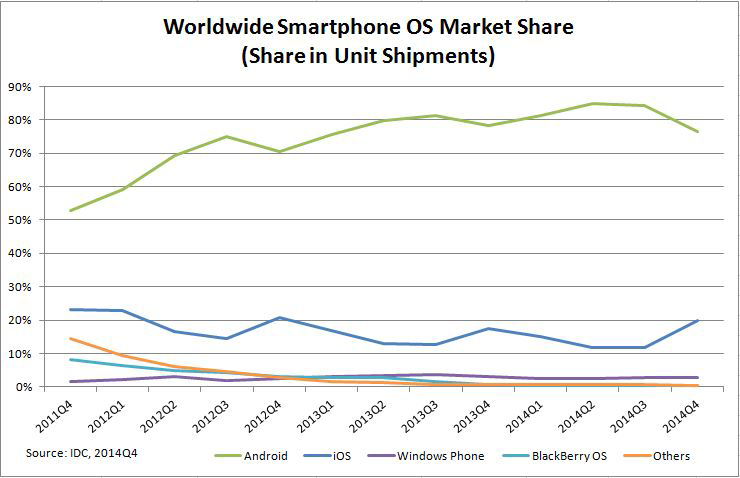
\includegraphics[width=0.98\linewidth]{./images/smartphone-os-market-share.png}
  		\caption{Operating Systems}
  		\label{fig:OSMarketShare}
	\end{subfigure}
	\begin{subfigure}{.49\textwidth}
  		\centering
  		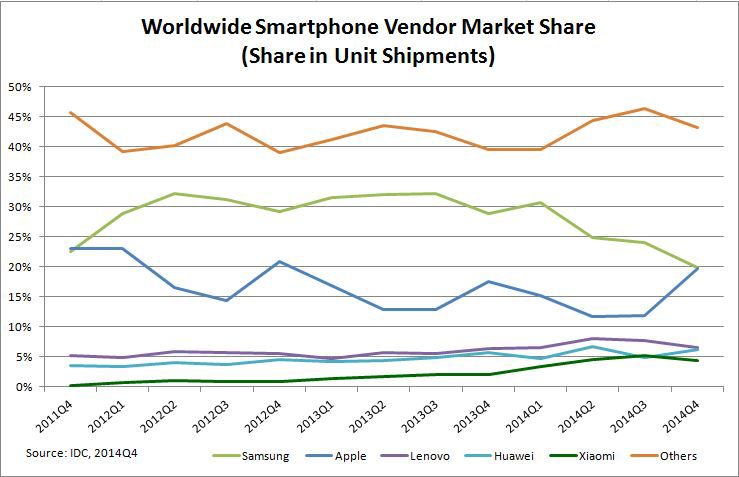
\includegraphics[width=0.98\linewidth]{./images/smartphone-vendor-market-share.png}
  		\caption{Vendors}
  		\label{fig:VendorMarketShare}
	\end{subfigure}
	\caption[Smartphone operating system's and vendor's market share, Q4 2014, retrieved from \cite{IDC:2015aa} and \cite{IDC:2015ab}]{Smartphone market share, Q4 2014}
	\label{fig:Shares}
\end{figure}
\nocite{IDC:2015aa, IDC:2015ab}

As shown in the last paragraph the importance of mobile applications rose tremendously within the last couple of years. Therefore it is essential to take this platform into consideration. When looking at the market shares of mobile \acrlong{OS}, shown in figure \vref{fig:OSMarketShare}, it seems obvious that an application should initially be developed for the \emph{Android} platform, since it got a market share of 76.6\% \cite{IDC:2015aa}. Later the development for \emph{iOS} (19.7\%) and \emph{Windows Phone} (2.8\%) might be considered \cite{IDC:2015aa}. But when looking at vendor market shares, shown in figure \vref{fig:VendorMarketShare}, this picture is not so obvious anymore. \emph{Apple}, the only vendor distributing devices with the \emph{iOS} \acrlong{OS}, has nearly the same market share as \emph{Samsung}, the biggest vendor of \emph{Android} running mobile devices \cite{IDC:2015ab}.

\begin{figure}[h]
	\centering
	\begin{subfigure}{.49\textwidth}
  		\centering
  		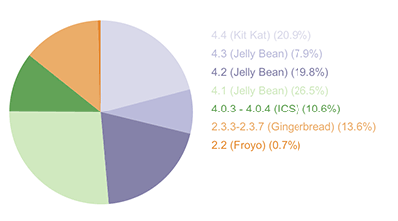
\includegraphics[width=0.98\linewidth]{./images/android-os.png}
  		\caption{Android}
  		\label{fig:AndroidOSFragmentation}
	\end{subfigure}
	\begin{subfigure}{.49\textwidth}
  		\centering
  		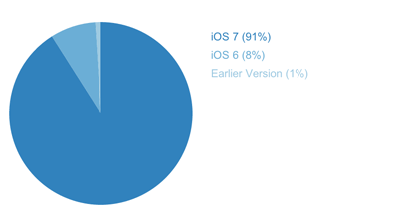
\includegraphics[width=0.98\linewidth]{./images/ios-os.png}
  		\caption{iOS}
  		\label{fig:iOSOSFragmentation}
	\end{subfigure}
	\caption[Mobile \acrfull{OS} fragmentation, retrieved from \cite{OpenSignal:2014aa}]{Mobile \acrfull{OS} fragmentation}
	\label{fig:MobileOSFragmentation}
\end{figure}
\nocite{OpenSignal:2014aa}

As already hinted, the \emph{Android} platform seems more fragmented than the \emph{iOS} eco-system. This is due to the fact that the \acrlong{OS} is distributed by several vendors, which create device with different specification. On top of that the support for the latest version of the \acrshort{OS} is not guaranteed, which not only leaves devices open for security vulnerabilities, but also increases the workload for the developer. As shown in figure \vref{fig:MobileOSFragmentation}, nearly 99\% of the \emph{iOS} devices were running the two latest versions of the \acrlong{OS} in 2014. In opposite to that, not even 50\% of the \emph{Android} devices were running the three latest revisions of the platform. This fragmentation is also reflected by figure \vref{fig:MobileScreenFragmentation}, which is showing all screen sizes of mobile devices running \emph{Android}, respectively \emph{iOS}, as of 2014.

\begin{figure}[h]
	\centering
	\begin{subfigure}{.49\textwidth}
  		\centering
  		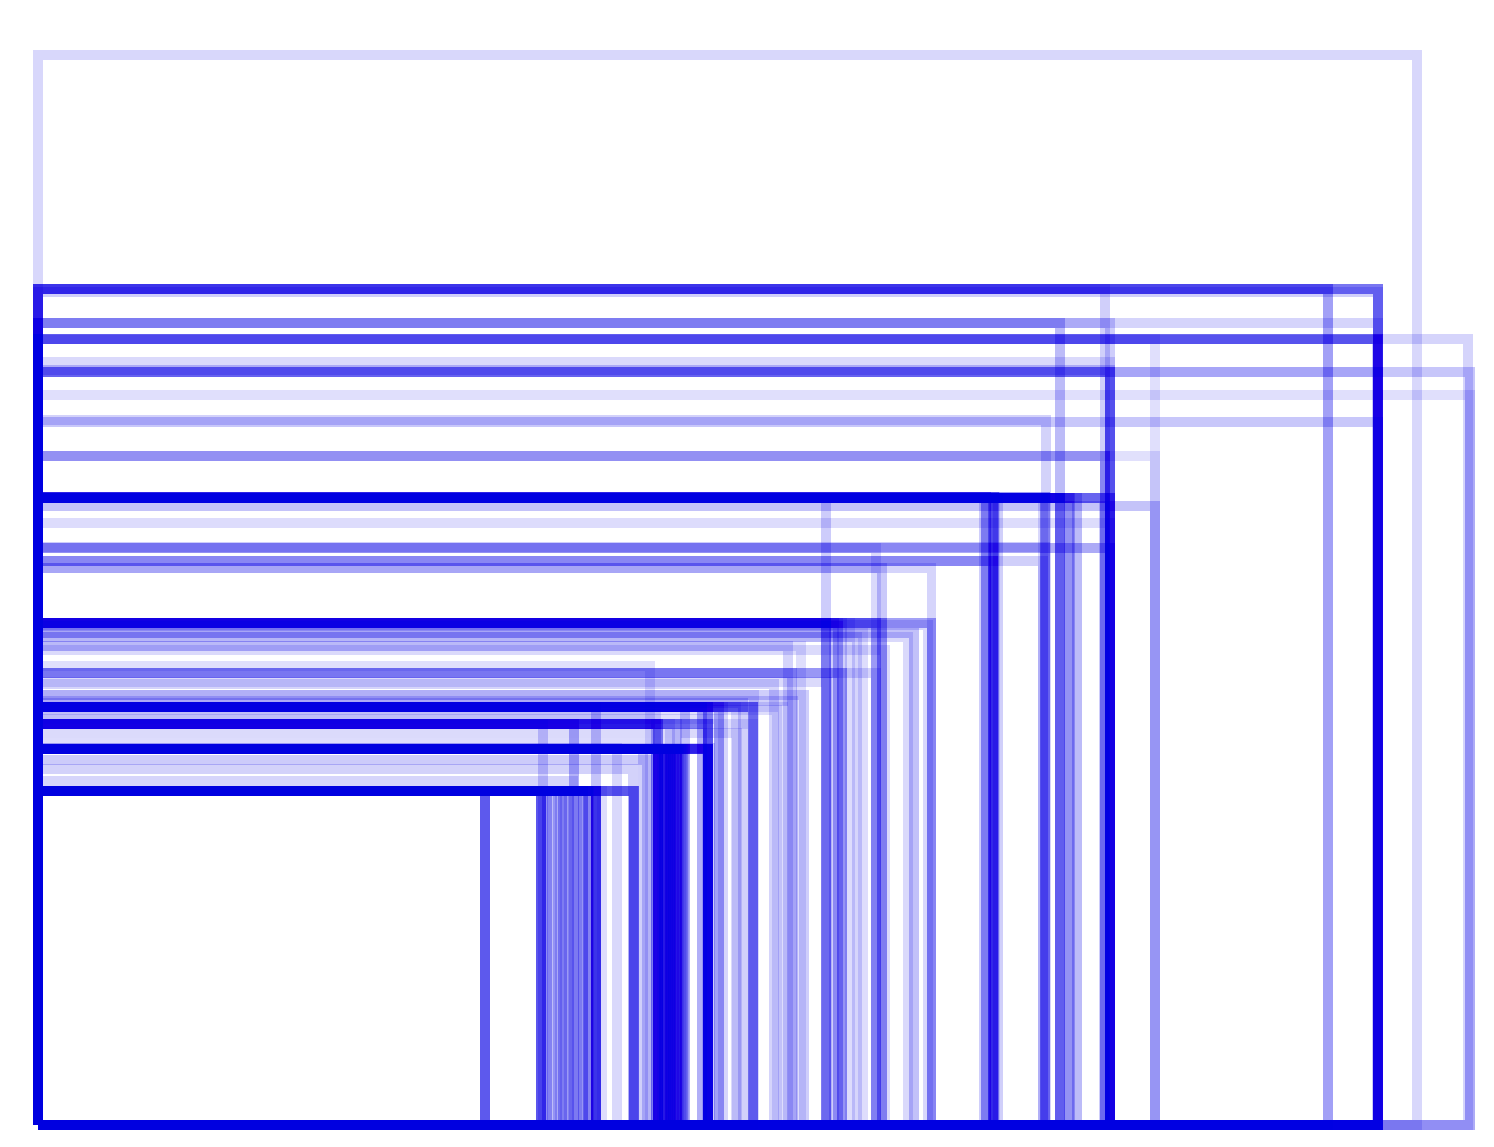
\includegraphics[width=0.98\linewidth]{./images/android-screen.png}
  		\caption{Android}
  		\label{fig:AndroidScreenFragmentation}
	\end{subfigure}
	\begin{subfigure}{.49\textwidth}
  		\centering
  		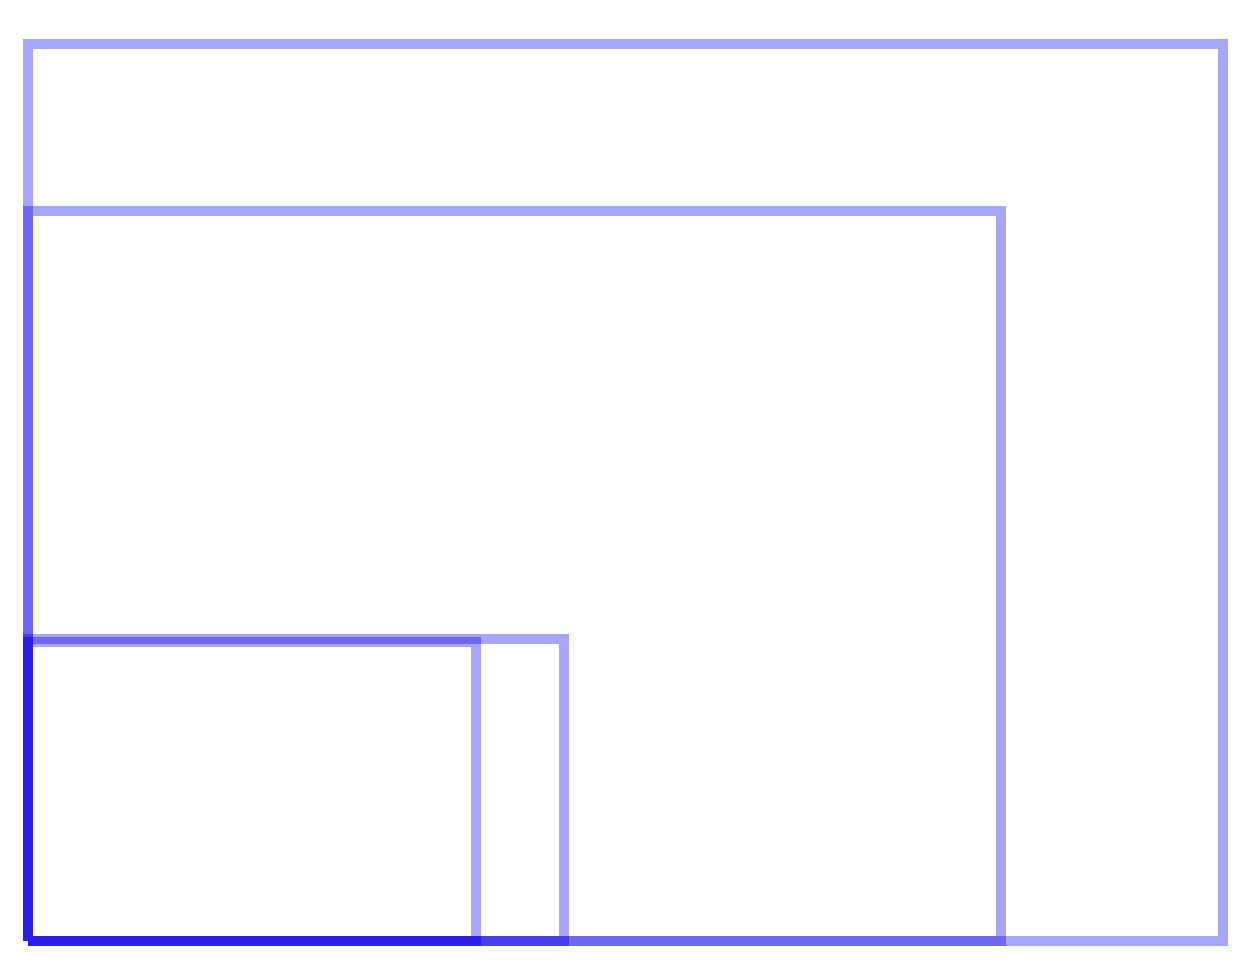
\includegraphics[width=0.98\linewidth]{./images/ios-screen.png}
  		\caption{iOS}
  		\label{fig:iOSScreenFragmentation}
	\end{subfigure}
	\caption[Screen size fragmentation of mobile devices grouped by \acrfull{OS}, retrieved from \cite{OpenSignal:2014aa}]{Screen size fragmentation of mobile devices grouped by \acrfull{OS}}
	\label{fig:MobileScreenFragmentation}
\end{figure}
\nocite{OpenSignal:2014aa}

Concluding, when creating an app for the \emph{Android} platform, the developer is facing several design decisions, which either increase the complexity of the program or reduce its functionality or accessibility. In opposite to that a developer choosing the \emph{iOS} platform can easily create an application which is optimised for all available devices, as well as exploiting all recent features offered by the \acrlong{OS} without excluding a big amount of users, who are not running on the latest version. 

Another decision that needs to be made is the amount of functionalities available on the different platforms. Eventually it is smarter to restrict certain functionalities to a platform or technology. This might decrease the complexity of a single application, but increase the development complexity.

In opposite of creating an application that includes all functionalities offered by the system there might be a dedicated application for administrative tasks and a member related tasks. This would reduce the complexity of the application for an administrator 


\section{Architecture} % Mapping to deployment model/ER model/architectural overview

\section{Functionality} %Mapping to final use cases

A brief wrap up and explanation of the key functionalities was given in chapter \vref{chapter:SellingPoint}. 

\section{User Interface} %% Mapping to wireframes

\chapter{Design}
(Wie kann ich mir es in der Umsetzung vorstellen, konzeptionelle umsetzung, wireframes, uml)

Requirements
Deployment model/Architectural model
Wireframes

Use case

\chapter{Implementation}
Umsetzung (Wie sieht es am ende aus, besonderheiten, tests aus entwurf -> Def aus pflichtenheft)

\section{UI}
color, logo, GUI

\section{Technical implementation}

fancy features

\chapter{Ongoing work}
\label{chapter:OngoingWork}
ausblick (max 1/8 vom text)

